\section{LQR controller with payload}
\subsection{full-state feedback controller}

The controller is constructed in Simulink (Figure~\ref{fig:simulink diagram full-state feedback controller}) according to the diagram on page 221 of the course notes. 

\begin{figure}[H]
	\centering
	\includegraphics[width=0.5\textwidth]{./LQG/full_state_feedback_simu.png}
	\caption{simulink diagram full-state feedback controller}
	\label{fig:simulink diagram full-state feedback controller}
\end{figure}

The matrix K is calculate with the LQR method as we did in the second exercise session. However in order to do LQR we need a matrix Q and R. As LQR minimizes $J_N = \frac{1}{2} \sum_{k=0}^{N-1}[x_k^TQx_k + u^T_kRu_k] + \frac{1}{2}x_N^TQx_N$. Notice how Q determines the weights given to $x_k$ and and R determines the weights given to $u_k$. 

If Q and R are taken as an diagonal matrix with ones on the diagonal then the quad copter does not have enough power to stay in the air. This is displayed in Figure~\ref{fig:full-state controller with simple diagonal matrices as Q and R}. Its very clear from Figure~\ref{fig:full-state controller with simple diagonal matrices as Q and R demo bad z position} that the controller does not optimize enough on the z axis.

\begin{figure}[H]
	\centering
	\begin{subfigure}[b]{0.3\textwidth}
		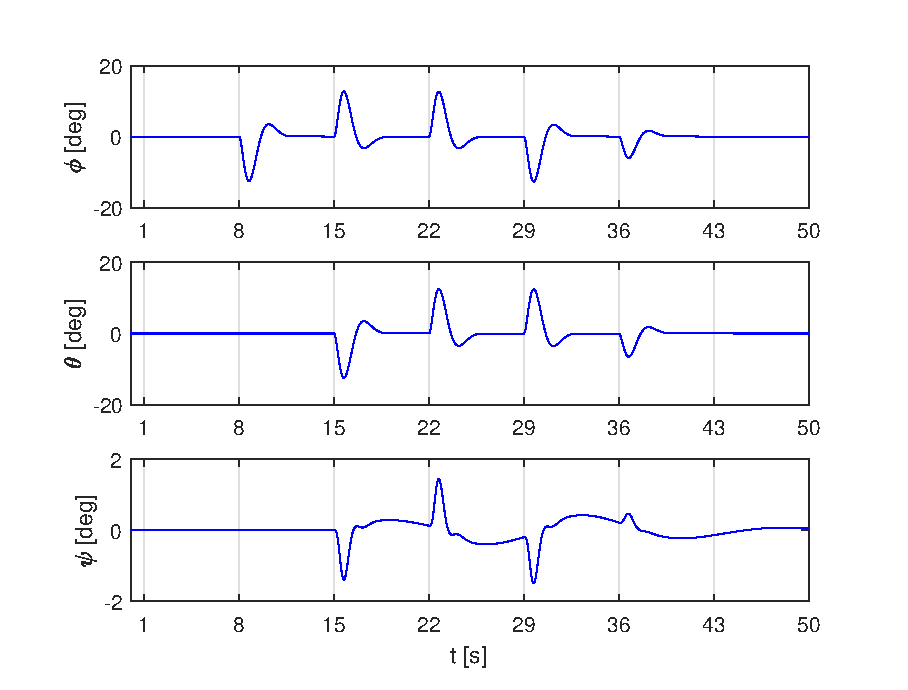
\includegraphics[width=\textwidth]{./LQG/full_state_feedback_first_fig4.eps}
		\caption{angels}
	\end{subfigure}
	\begin{subfigure}[b]{0.3\textwidth}
		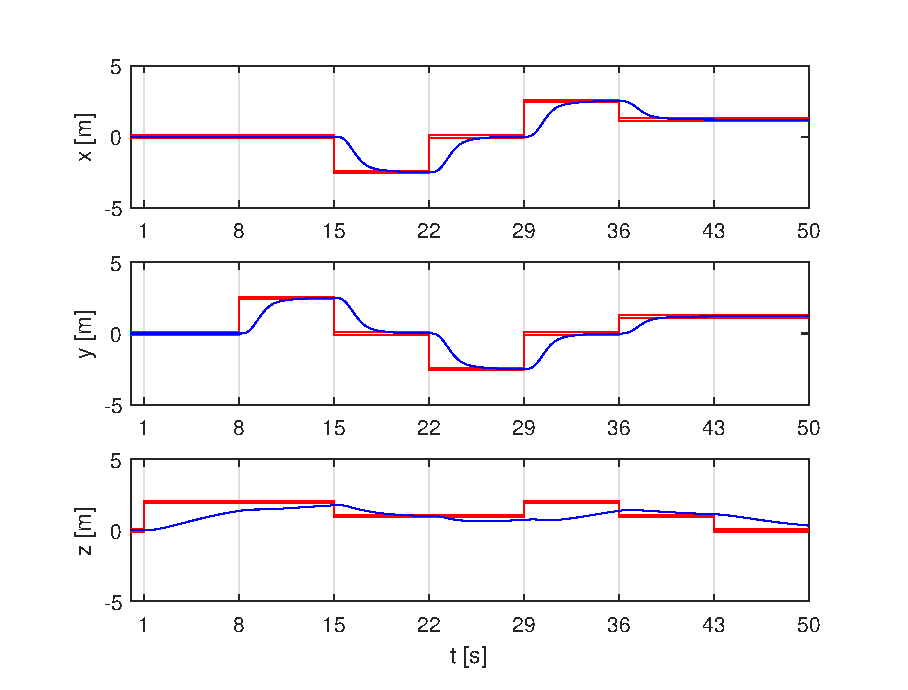
\includegraphics[width=\textwidth]{./LQG/full_state_feedback_first_fig3.eps}
		\caption{position}
		\label{fig:full-state controller with simple diagonal matrices as Q and R demo bad z position}
	\end{subfigure}
	\begin{subfigure}[b]{0.3\textwidth}
		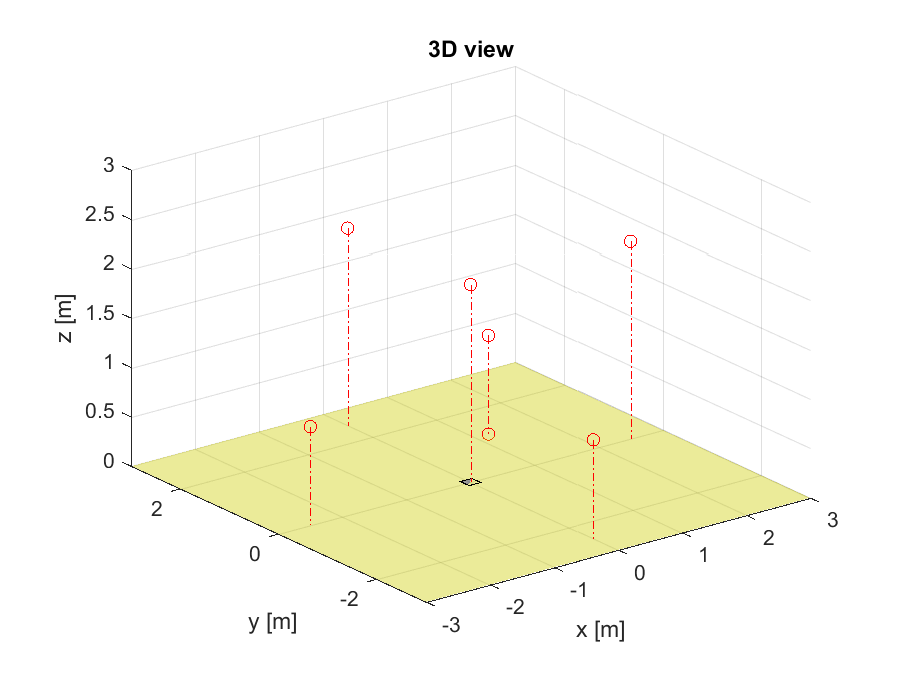
\includegraphics[width=\textwidth]{./LQG/full_state_feedback_first_fig2.eps}
		\caption{position}
	\end{subfigure}
	\caption{full-state controller with simple diagonal matrices as Q and R}\label{fig:full-state controller with simple diagonal matrices as Q and R}
\end{figure}

In order to get a proper controller we need to put way more weight on the position z in the optimization problem. This is done by increasing a value in Q, as the z coordinate is an state. 

$$ 
Q=
\begin{bmatrix}
1 & 0 & 0 & ... \\
0 & 1 & 0 & ...\\
0 & 0 & 1 & ... \\
... & ... & ... & ... 
\end{bmatrix}
=>
\begin{bmatrix}
1 & 0 & 0 & ...\\
0 & 1 & 0 & ...\\
0 & 0 & 10^{7} & ... \\
... & ... & ... & ... 
\end{bmatrix}
$$

\begin{figure}[H]
	\centering
	\begin{subfigure}[b]{0.3\textwidth}
		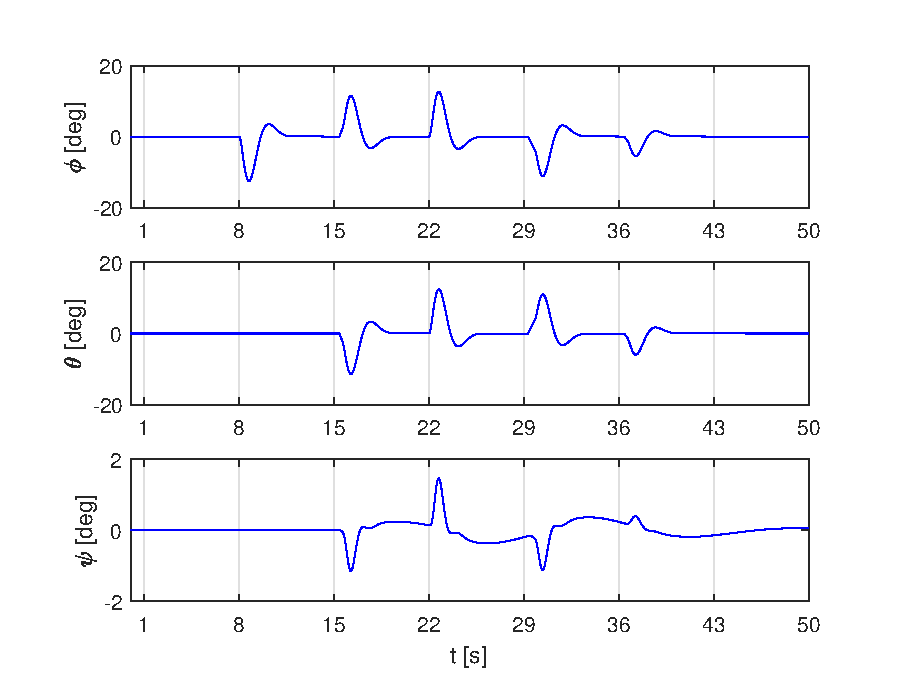
\includegraphics[width=\textwidth]{./LQG/full_state_feedback_final_fig4.eps}
		\caption{angels}
	\end{subfigure}
	\begin{subfigure}[b]{0.3\textwidth}
		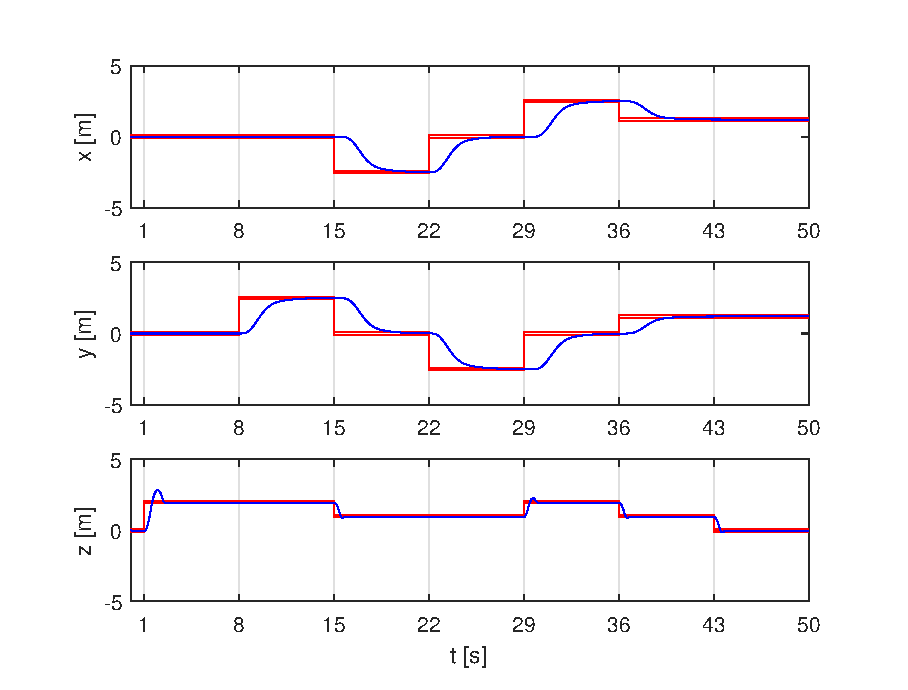
\includegraphics[width=\textwidth]{./LQG/full_state_feedback_final_fig3.eps}
		\caption{position}
	\end{subfigure}
	\begin{subfigure}[b]{0.3\textwidth}
		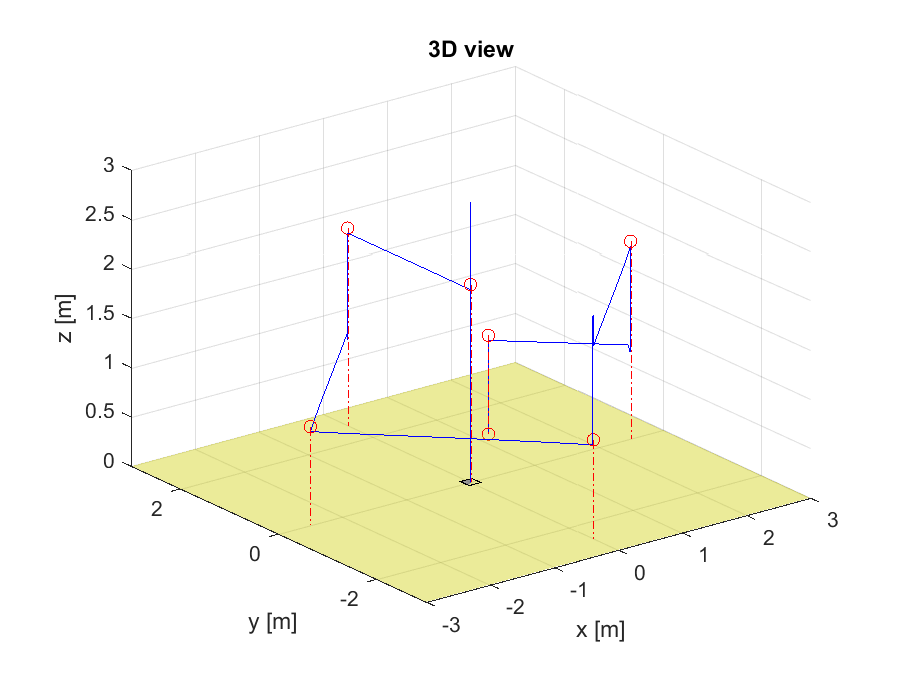
\includegraphics[width=\textwidth]{./LQG/full_state_feedback_final_fig2.eps}
		\caption{position}
	\end{subfigure}
	\caption{full-state controller with proper diagonal matrices as Q and R}\label{fig:full-state controller with proper diagonal matrices as Q and R}
\end{figure}
\subsection{LQR controller with integral action}

\subsection{discussion both results}
\section{LQR controller without payload}
